\newpage
\section*{Energy Calibration}

An energy calibration of the three scintillator detectors was necessary in order to perform the experiment. The $\gamma$-sources used as reference were $^{241}$Am with a 59.5~keV photopeak, in order to have low energies values, and $^{22}$Na with two photopeak at 511~keV and 1275~keV.

The uncalibrated spectra obtained are shown in Fig.~\ref{Fig:Uncalibrated_spectra}:

\begin{figure}[h!]
	\centering
	\subfloat[][\emph{Detector $^{241}$Am  spectrum }.]
	{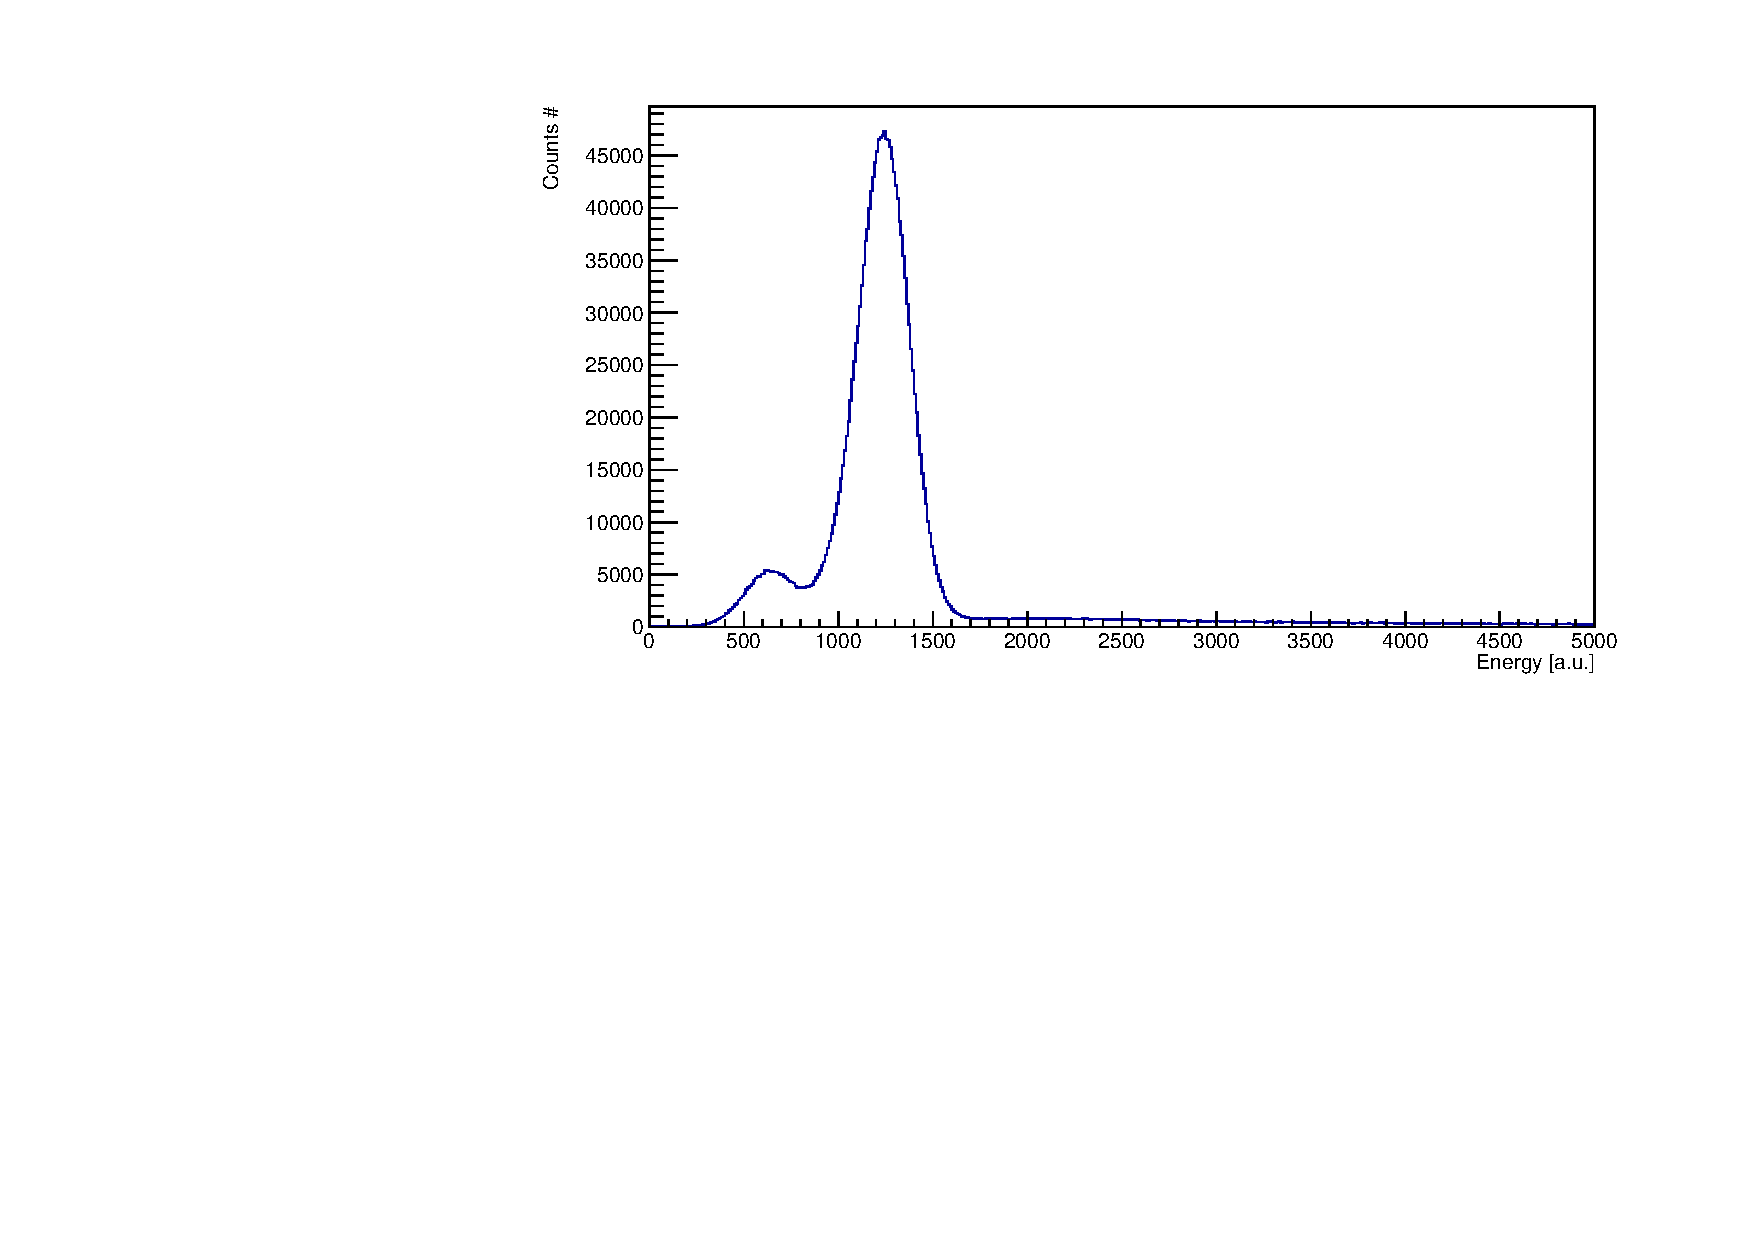
\includegraphics[width=.45\textwidth]{Detector_Am241}} \quad
	\subfloat[][\emph{Detector $^{22}$Na spectrum }.]
	{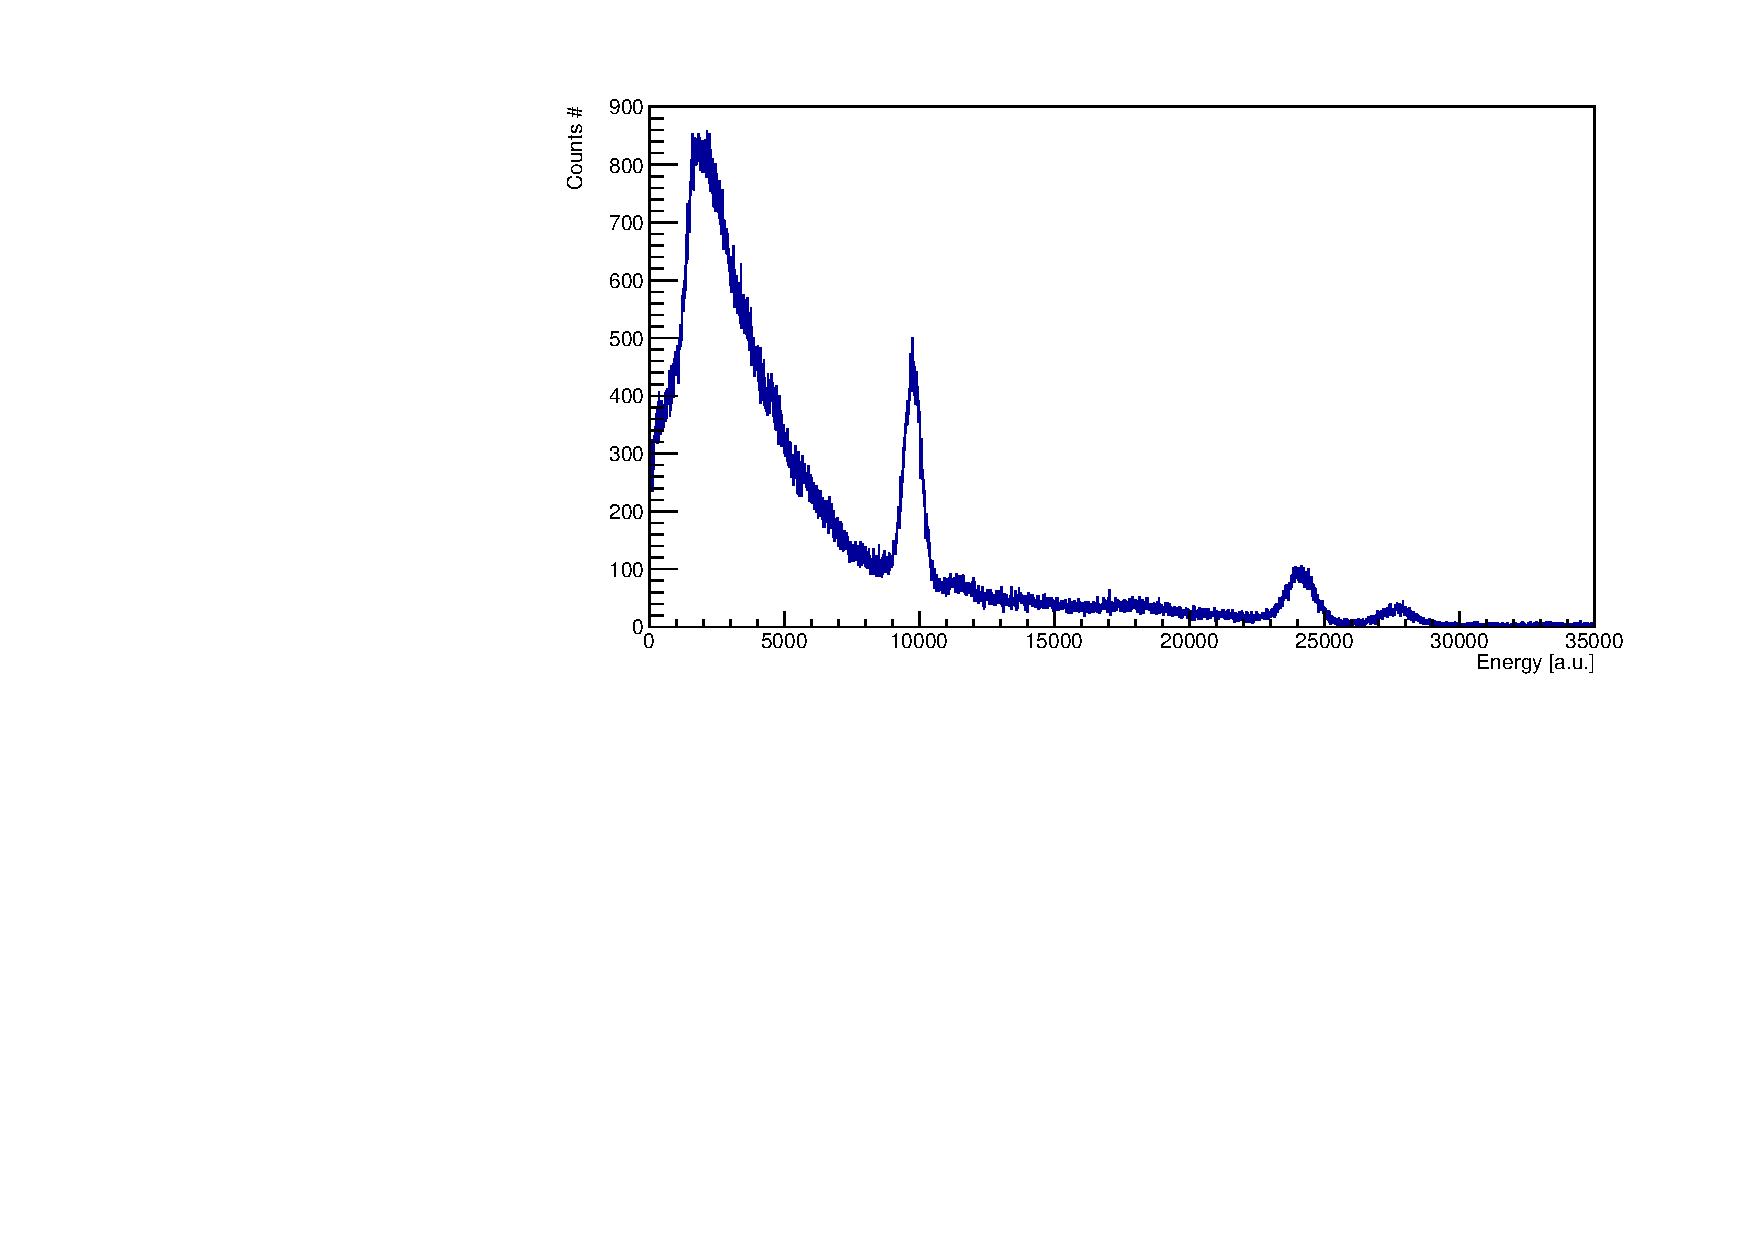
\includegraphics[width=.45\textwidth]{Detector_Na22}} \quad
	\subfloat[][\emph{Scatterer $^{241}$Am  spectrum }.]
	{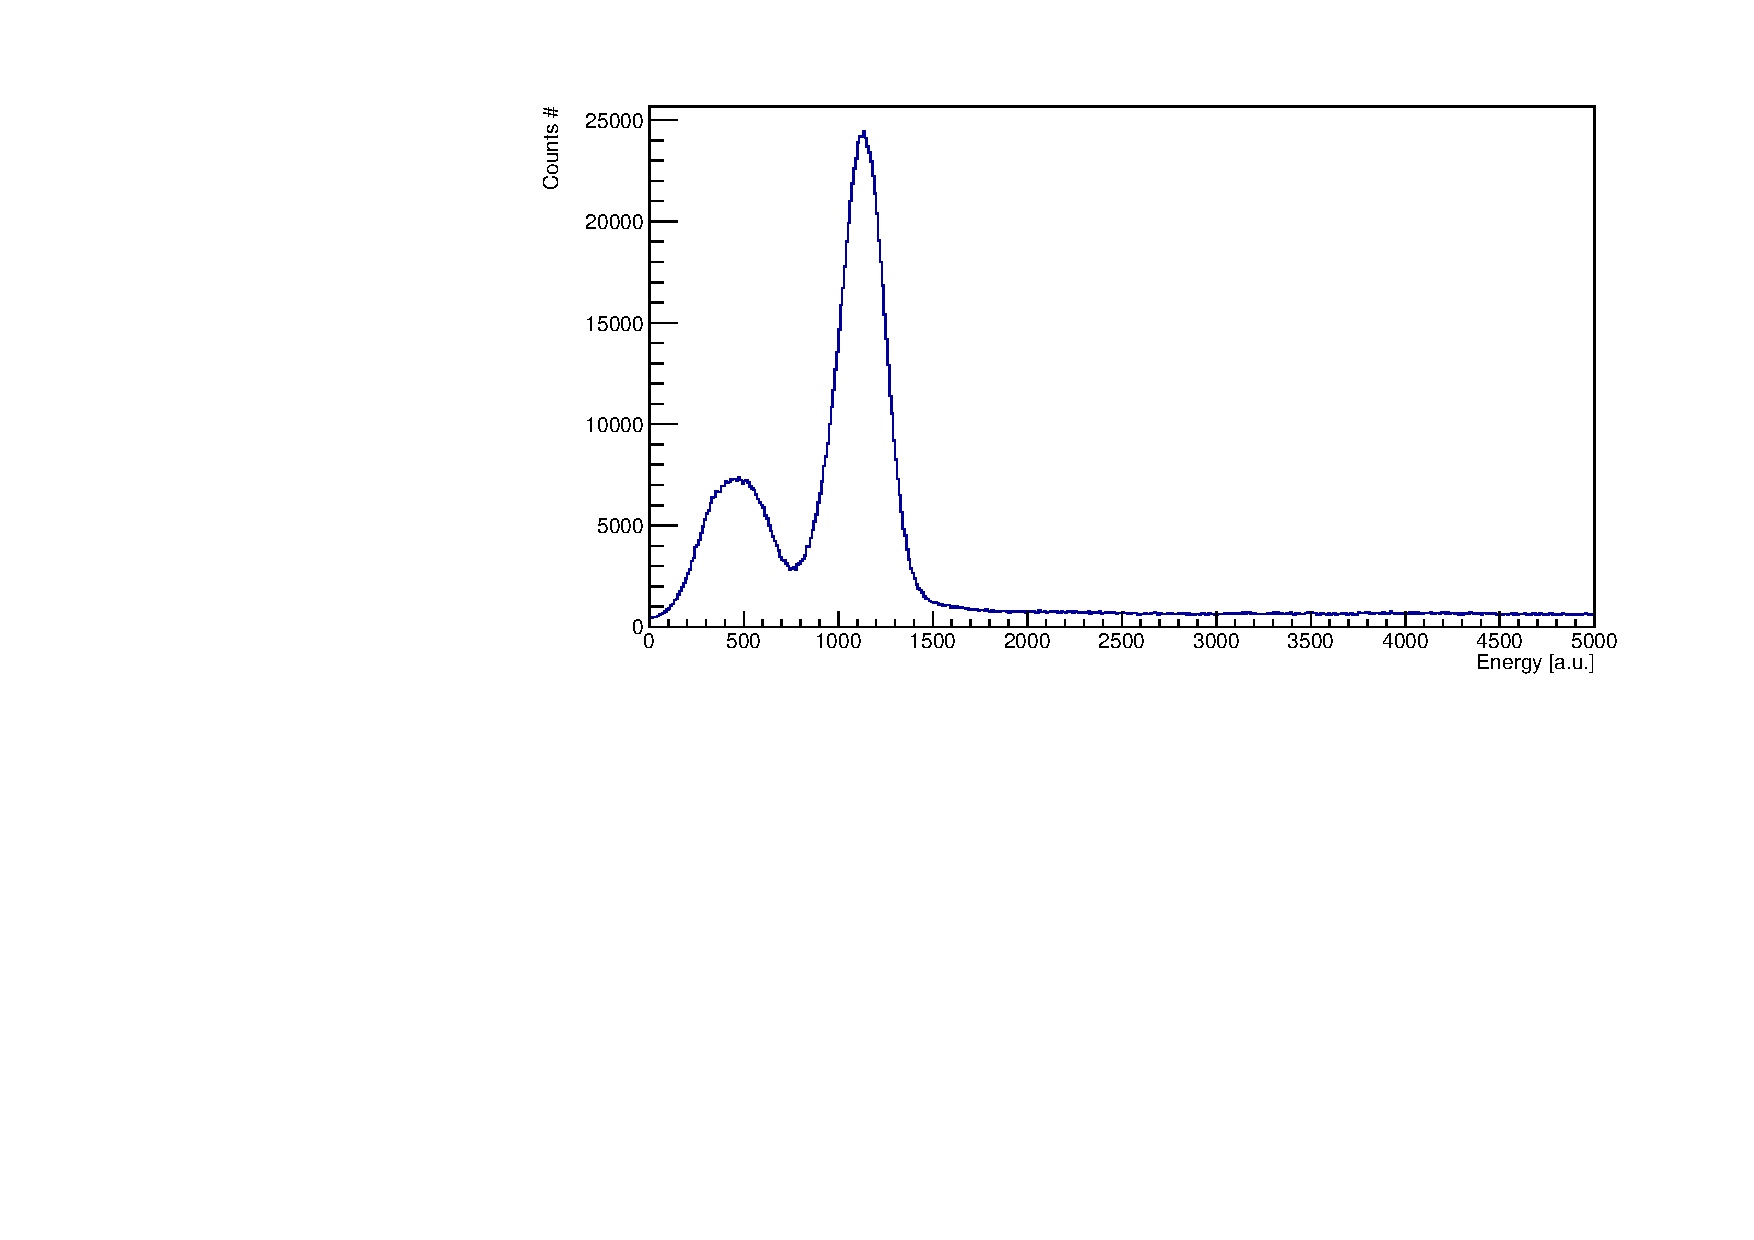
\includegraphics[width=.45\textwidth]{Scatterer_Am241}} \quad
	\subfloat[][\emph{Scatterer $^{22}$Na spectrum }.]
	{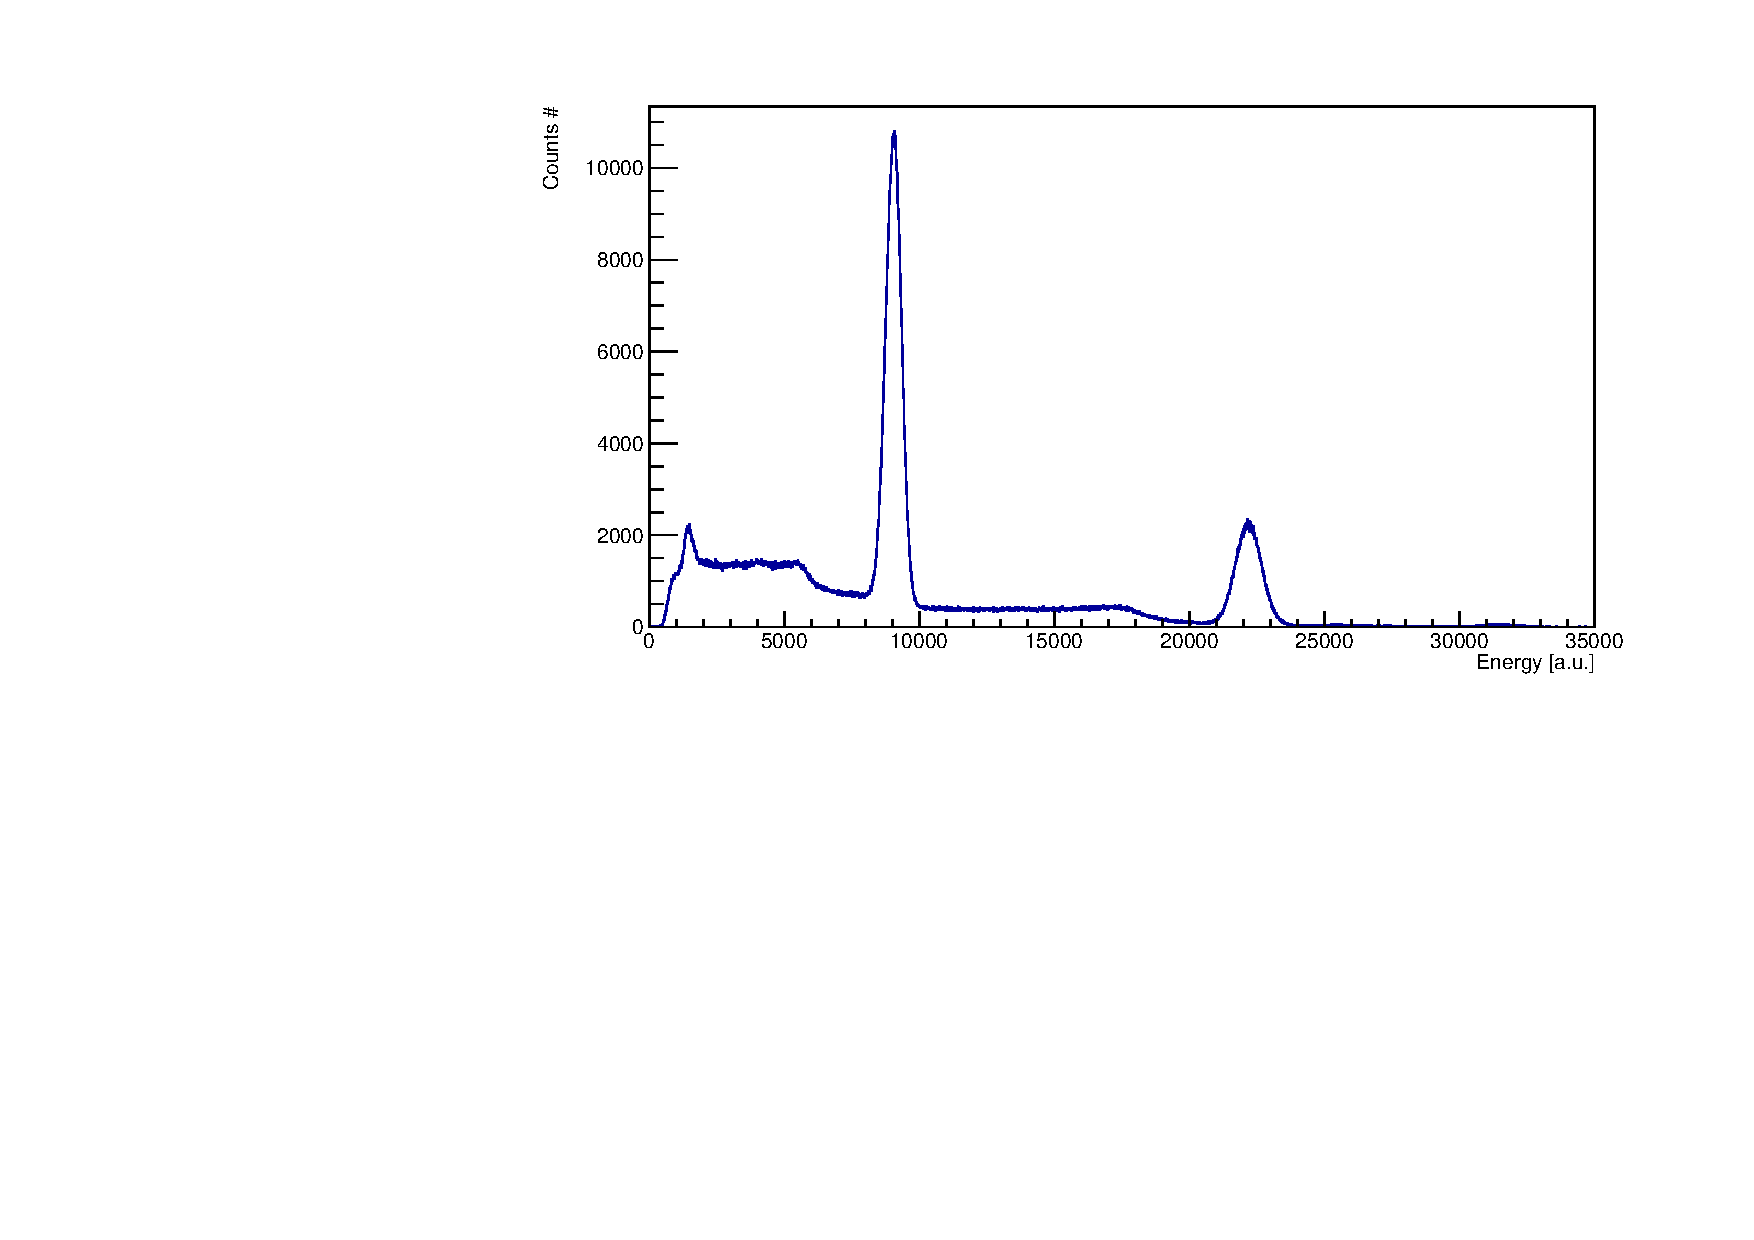
\includegraphics[width=.45\textwidth]{Scatterer_Na22}} \quad
	\subfloat[][\emph{Tagger $^{241}$Am  spectrum }.]
	{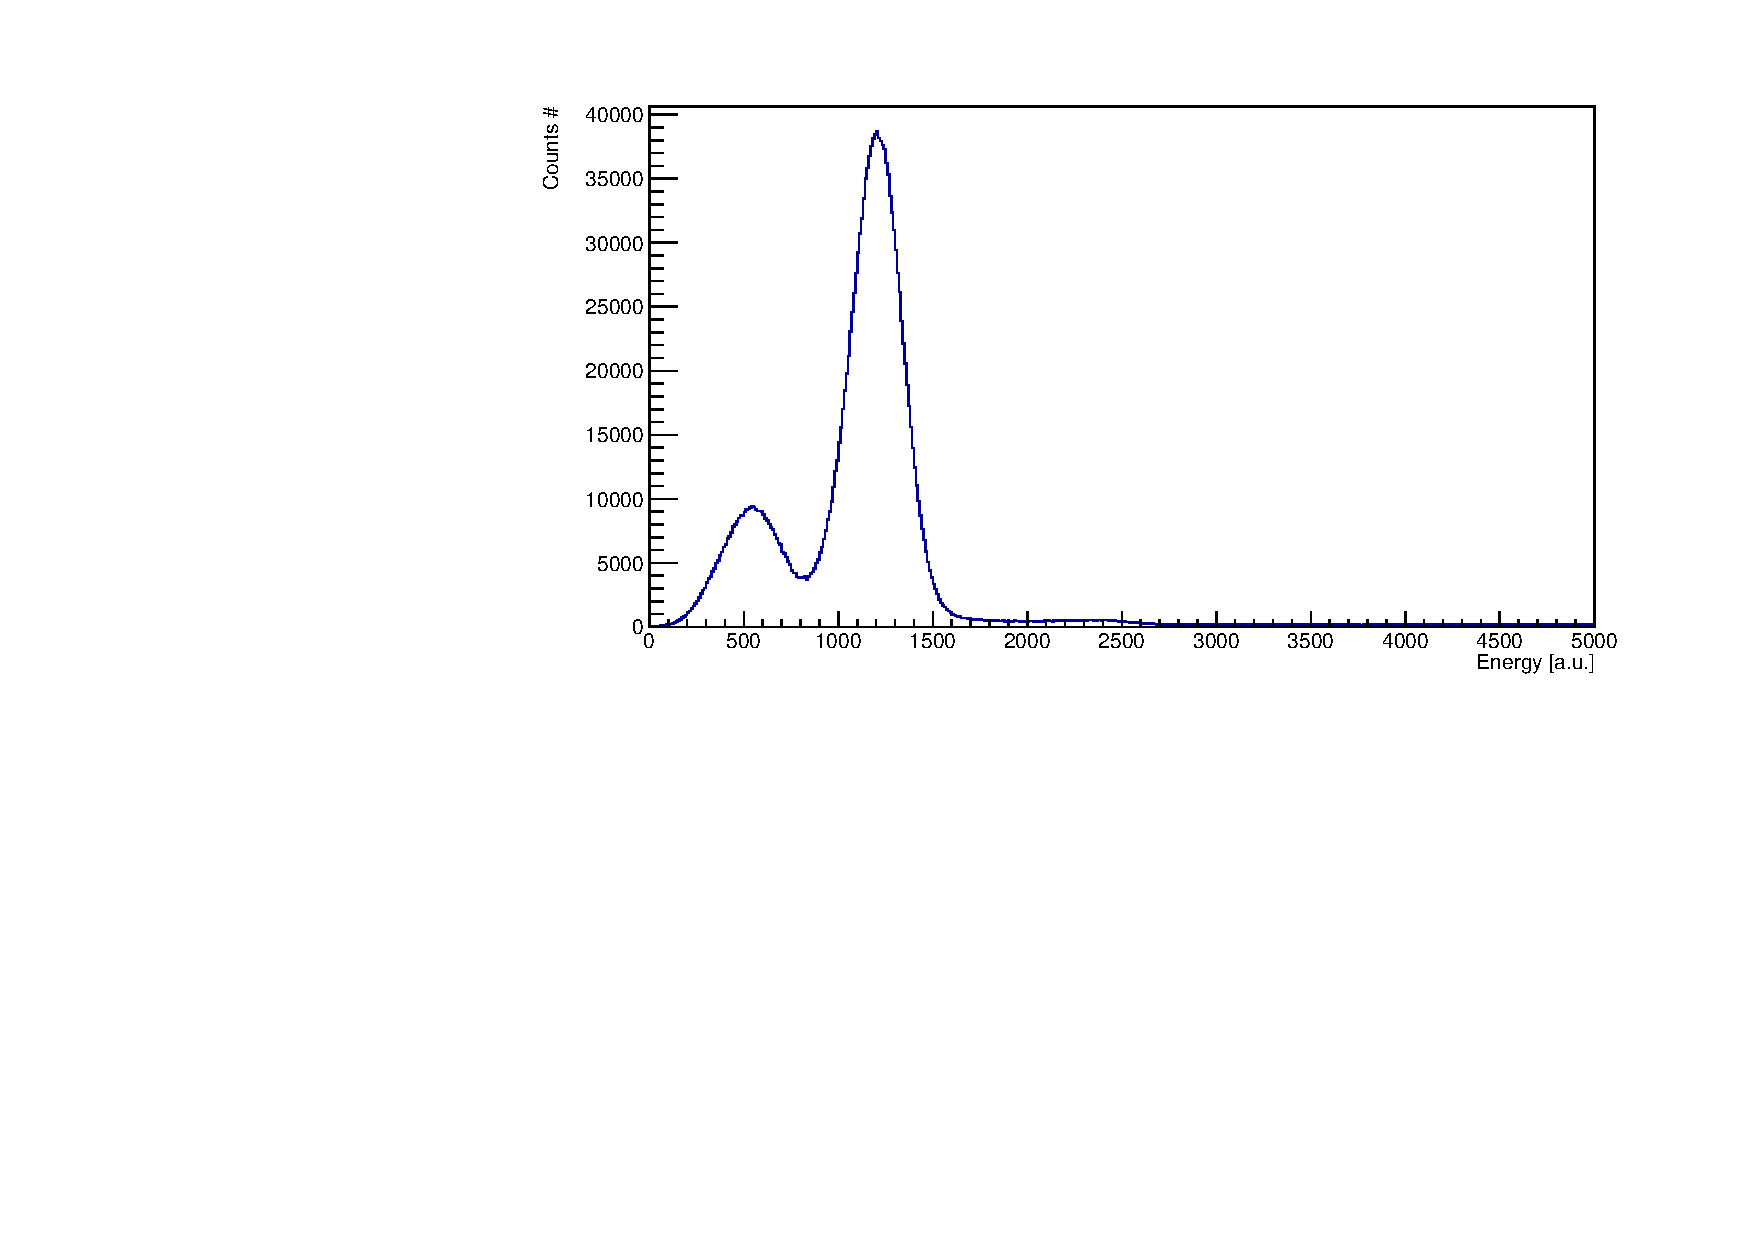
\includegraphics[width=.45\textwidth]{Tagger_Am241}} \quad
	\subfloat[][\emph{Tagger $^{22}$Na spectrum }.]
	{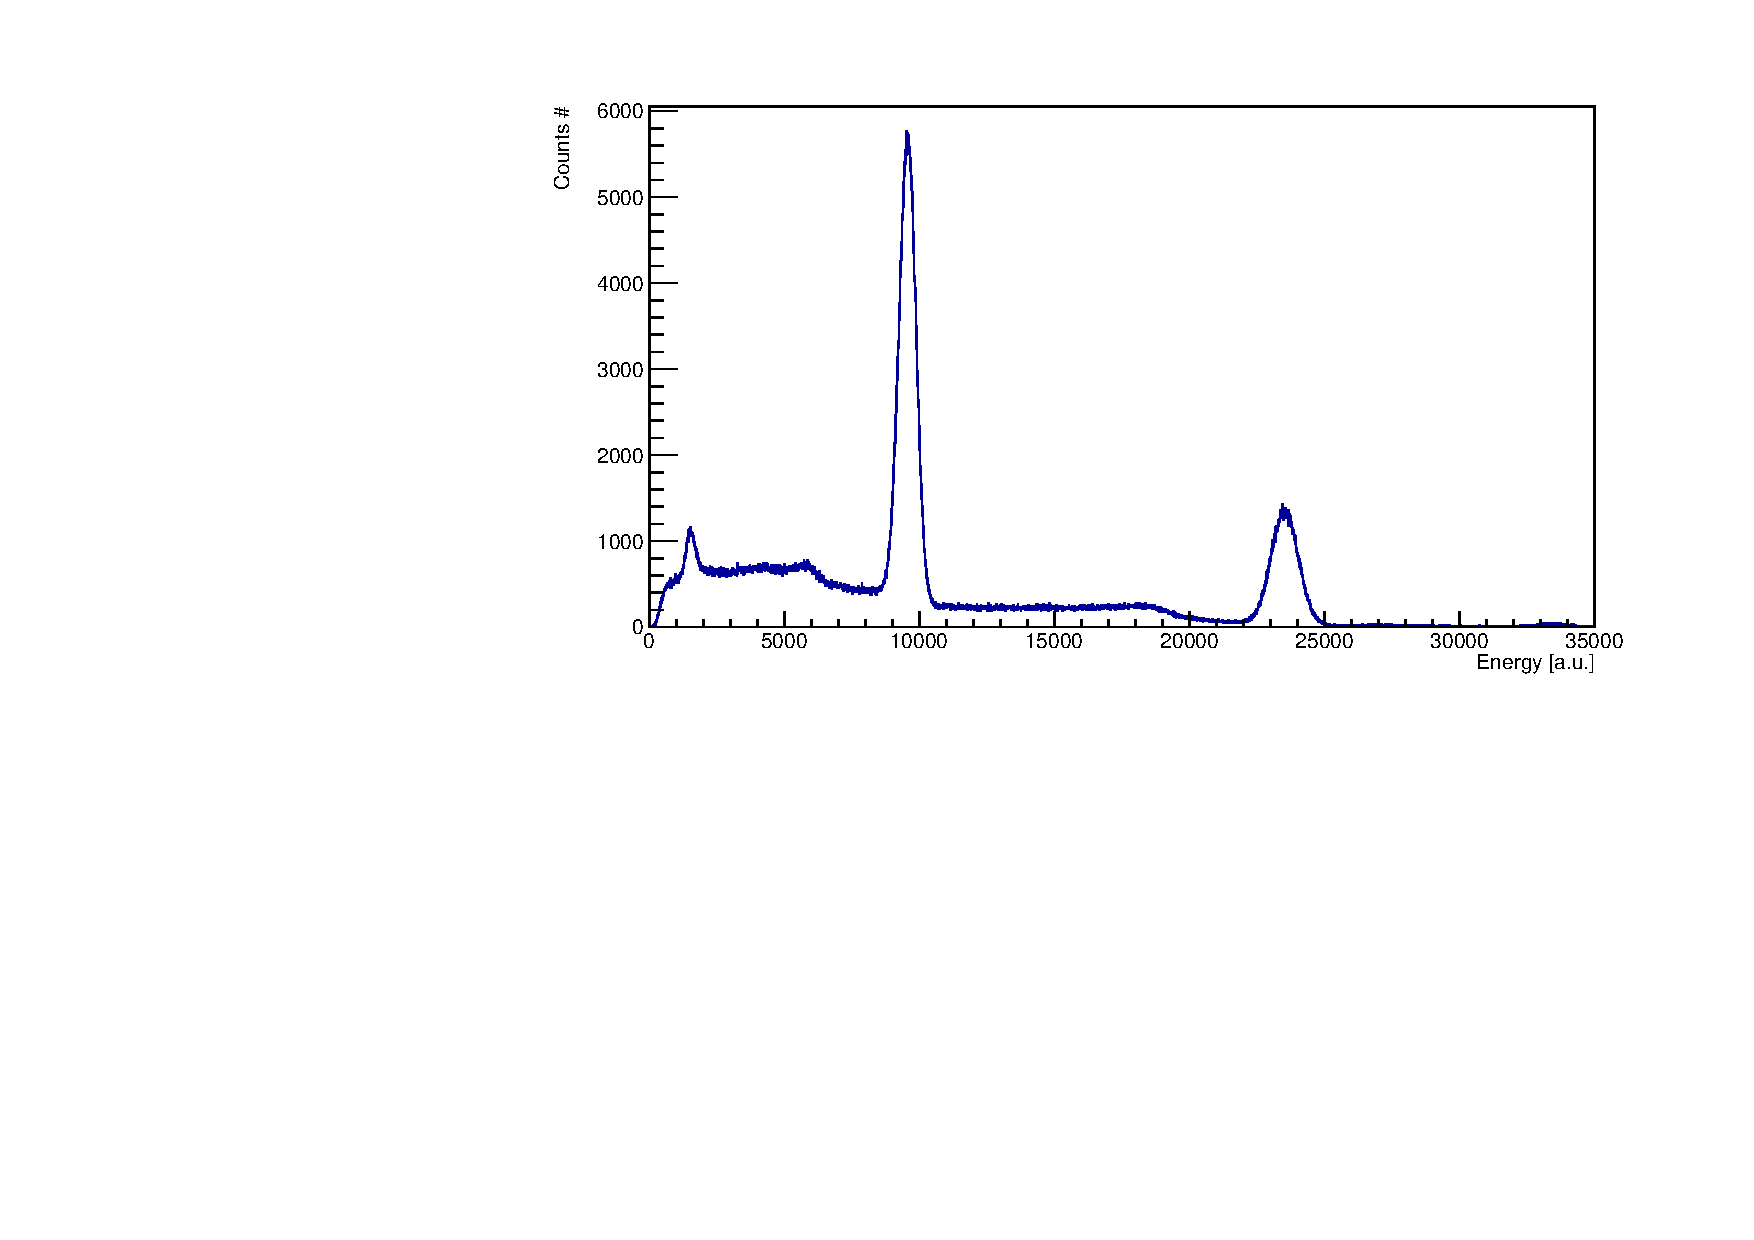
\includegraphics[width=.45\textwidth]{Tagger_Na22}} \\
	\caption{Uncalibrated spectra of the three detectors used in the experiment obtained with $^{241}$Am and $^{22}$Na $\gamma$-sources .}
	\label{Fig:Uncalibrated_spectra}
\end{figure}

The calibration parameters for the three detectors were found perfoming a linear interpolation between the three energy points and the corresponding uncalibrated peak centroids obtained with a Gaussian fit and are shown in Tab.~\ref{Tab:Calibration parameters}:

\begin{table}[H]
\centering
\begin{tabular}{c|cc}
\toprule
\toprule
 & P0~[keV] & P1~[keV/ch] \\
\midrule
Tagger & -6$\pm$1 &  0.54436$\pm$0.00006 \\
Scatterer & -8$\pm$4 & 0.0577$\pm$0.0003 \\
Detector & -7$\pm$1 & 0.05318$\pm$0.00007 \\
\bottomrule
\bottomrule
\end{tabular}
\caption{Calibration Parameters}
\label{Tab:Calibration parameters}
\end{table}